\chapter{Kísérlet}\label{chap:experiment}

Ebben a fejezetben a kísérleti összeállítás kerül bemutatásra. A motor összeállítás és a mérési eszközök 
részletes dokumentációja után az alkalmazott mérési és vezérlési módszerek sajátosságainak bemutatása 
következik. Ezután szabályozó viselkedésének elemzésére kerül sor az előző fejezetekben bemutatott modellel 
összehasonlítva.

\section{Mérési összeállítás}
A mérésekhez felhasznált egyenáramú motor egy maxon összeállítás része. Az összeállítás egy 
kis teljesítményű DC motorból, egy bolygókerekes hajtóműből és egy enkóderből áll. A motor paraméterei
az \ref{fig:motor_datasheet}. ábrán szereplő adatlapon találhatóak. A hajtómű és az enkóder leírása pedig 
a \ref{fig:gearhead_datasheet}. és \ref{fig:encoder_datasheet}. ábrákon láthatóak. A gravitáció hatásának 
kiküszöbölésére a mérésekhez a motort álló helyzetben kellett rögzíteni. Ehhez készült egy 3D nyomtatott 
műanyag keret, ami a hajtóműhöz csatlakozik. A teljes összeállítás az \ref{fig:setup_experiment}. ábrán 
látható. 
\begin{figure}[H]
    \begin{center}
    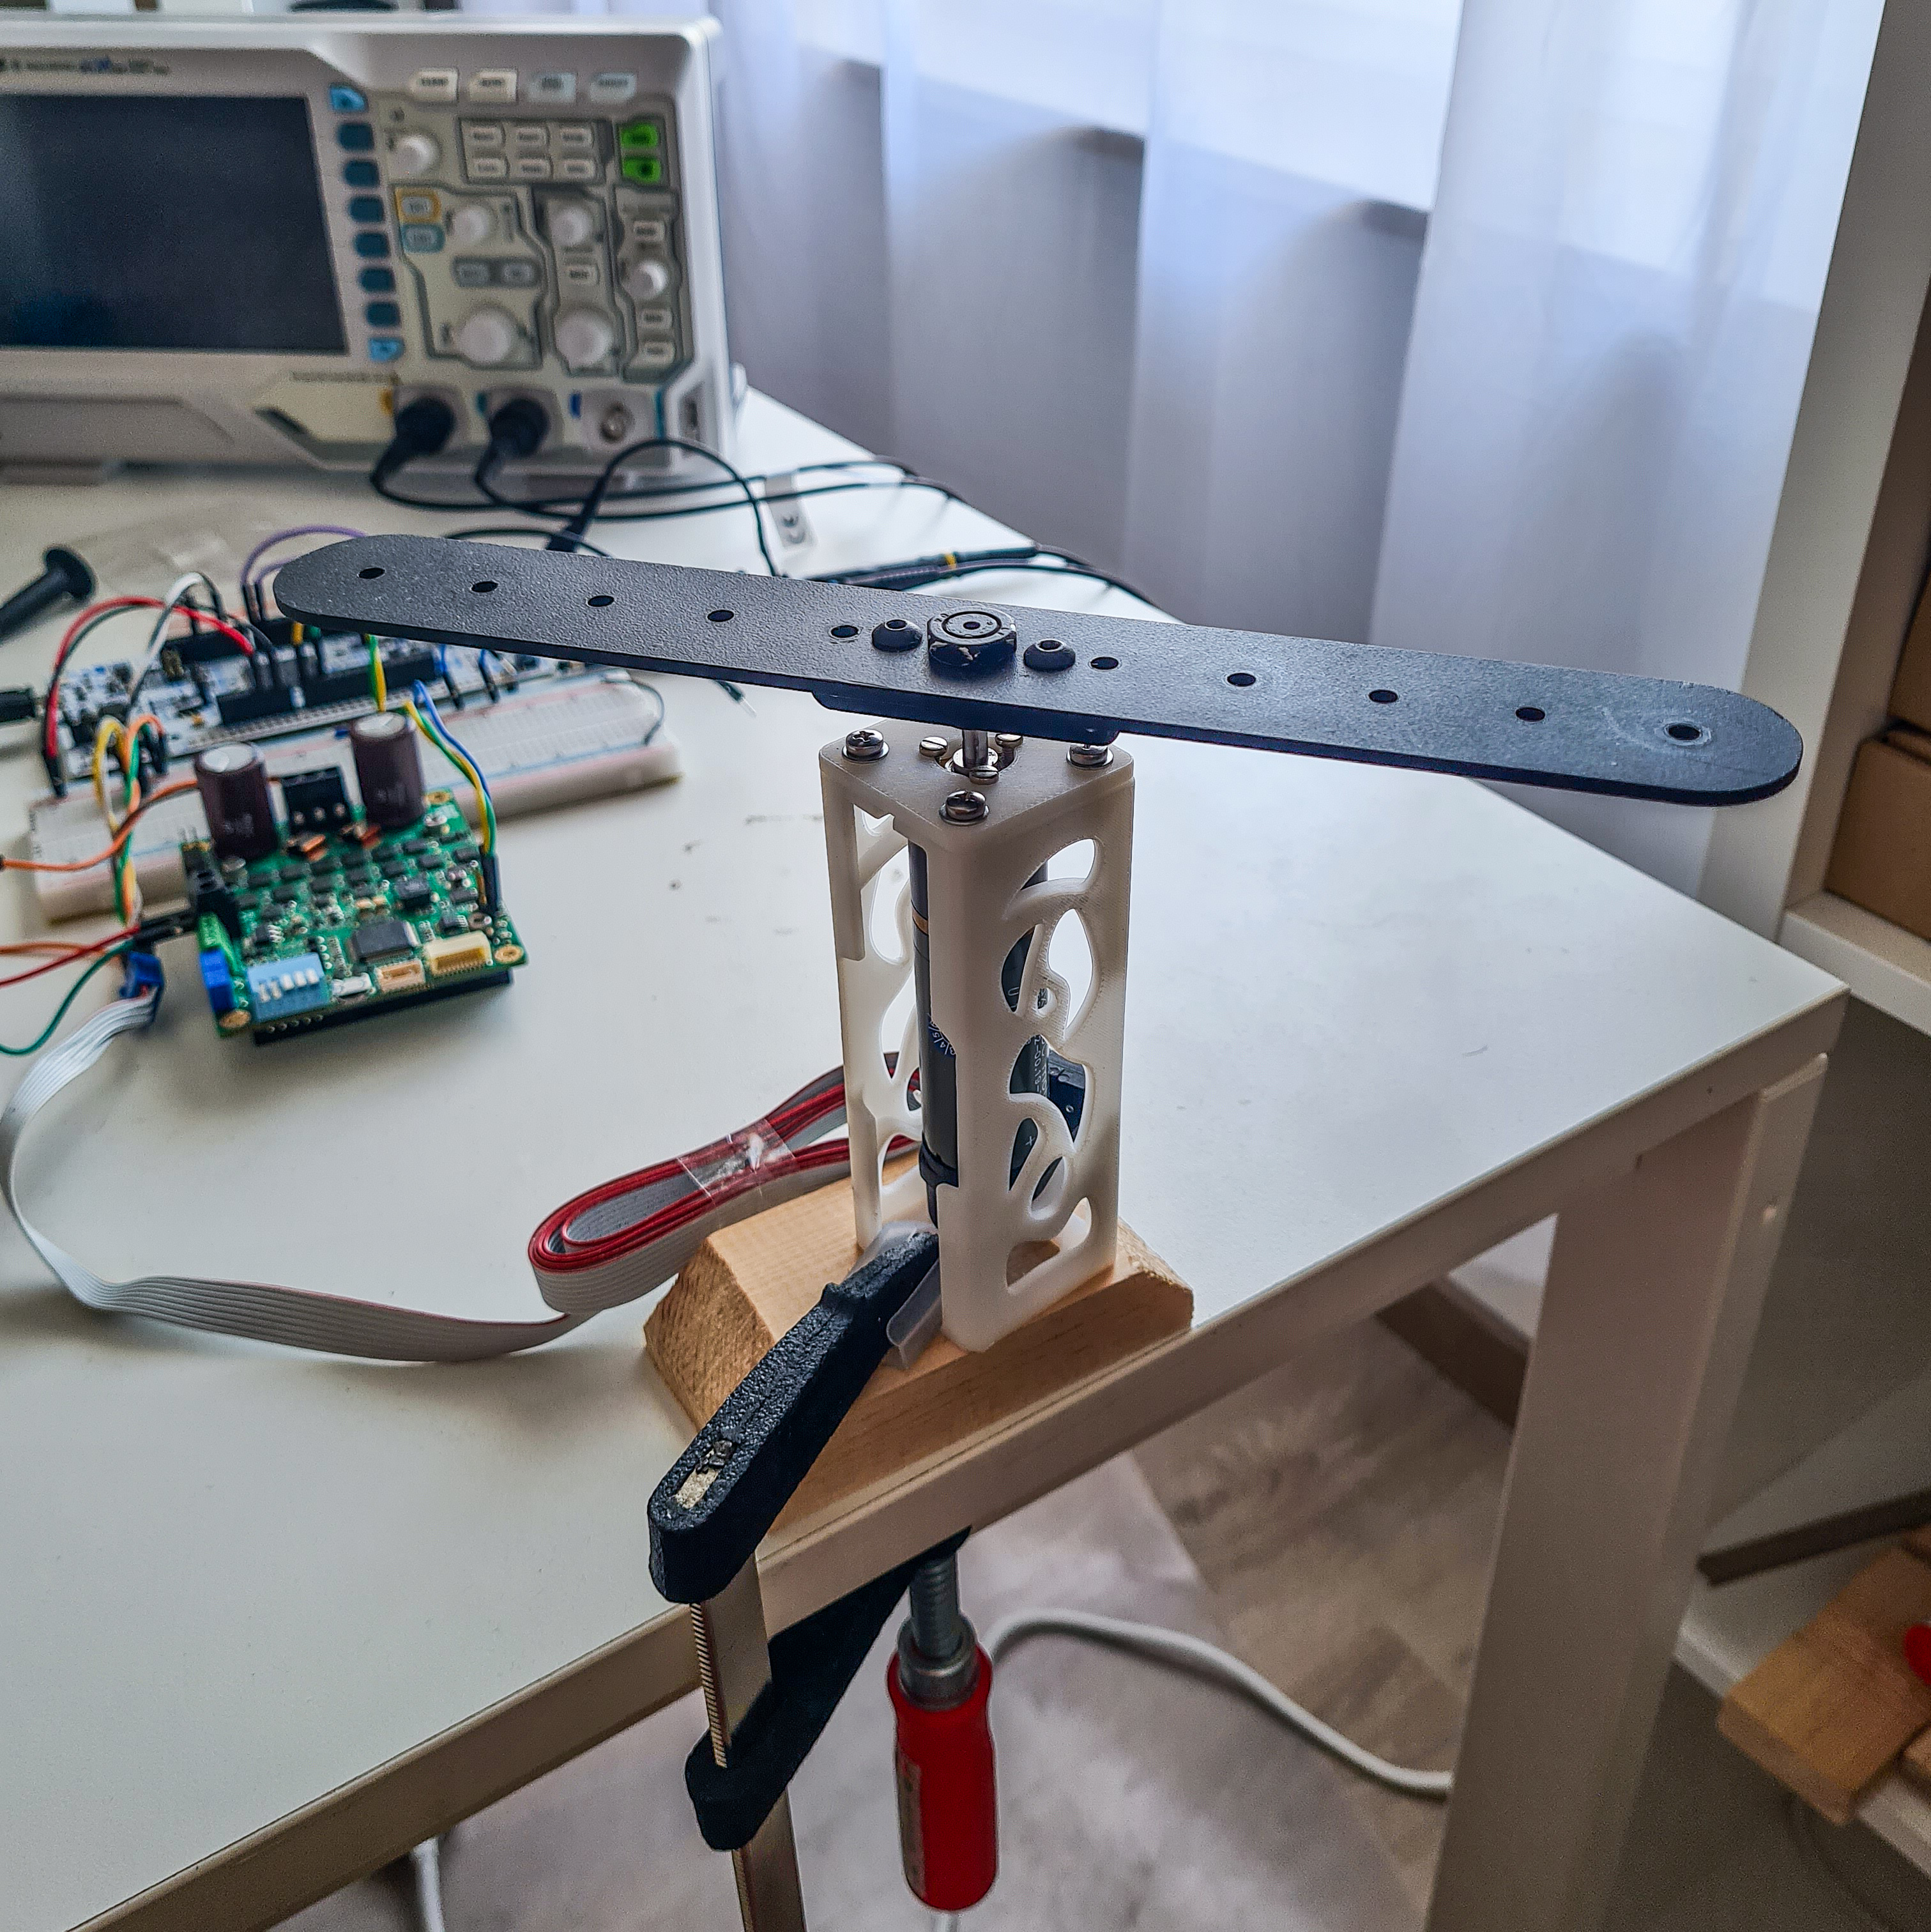
\includegraphics[width=14cm]{images/setup_experiment.jpg}
    \caption{Mérési összeállítás}\label{fig:setup_experiment}
    \end{center}
\end{figure}
A motorvezérlő egy SOLO UNO V2 32A típúsú univerzális vezérlő egység, mely egyenáramú kefés, kefe 
nélküli valamint PMSM és váltakozó áramú indukciós motorok vezérlésére is alkalmas 800W-ig. 
A kimenet változtatható frekvenciájú PWM jel. A kimeneti PWM vezérlő jel frekvenciája elméletben 80kHz-ig 
növelhető. A valóságban 75kHz-es beállítás felett automatikusan visszaugrott a frekvencia 20kHz-re, így 
a kísérletek során 75kHz volt a beállított frekvencia. CANopen és egy egyedi UART 
protokollon keresztül lehet kommunikálni az eszközzel. A kísérletek során a második opció lett alkalmazva.

% Alacsony induktivitású motoroknál, amilyen a kísérletben is felhasznált maxon motor, 
% a vezérlő jel átlagos amplitúdója és a motor nyomatéka között nem feltétlenül van lineáris kapcsolat. 
% Mivel ez egy alapvető feltétele a szabályozó alkalmazhatóságának, most ennek a jelenségnek a 
% részletesebb elemzése következik. A második fejezetben szereplő 
% \eqref{eq:rotor_dynamics} és \eqref{eq:armature_circuit} egyenletek alapján \dots

A szabályozó futtatását egy NUCLEO-F439ZI STMicrocontrollers fejlesztői panel végzi.
Alapvető feladatai:
\begin{itemize}
    \item Az inkrementális enkóder jelének olvasása a beépített számláló és időzítő periférián keresztül
    \item A szabályozó belső állapotának frissítése pontosan meghatározott időközönként.
    \item A szabályozó kimeneti referencia jelének továbbítása a motorvezérlőnek az előírt időkésés figyelembe vételével.
    \item A mérés állapotának felvétele és továbbítása a számítógép felé.
\end{itemize}
A szoftver egyszerűsített vázlata az \ref{fig:block_diagram_control_software}. ábrán látható. 
\begin{figure}[H]
    \begin{center}
    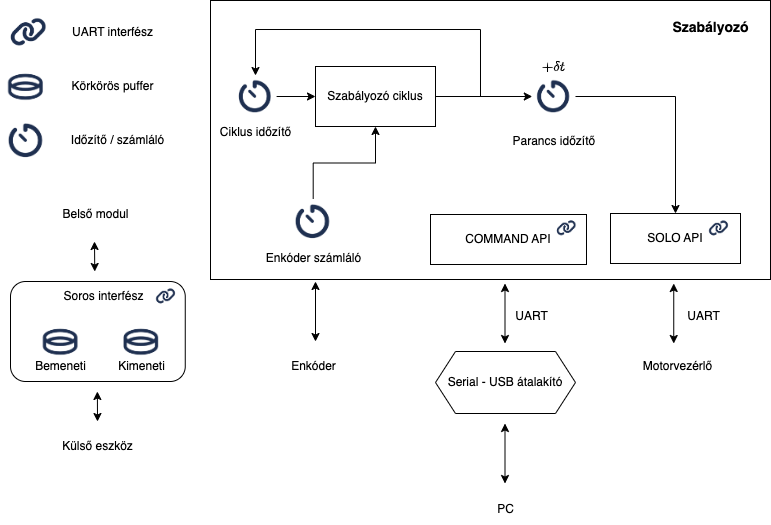
\includegraphics[width=14cm]{images/impedance_controler_software_diagram.png}
    \caption{Szabályozó szoftveres implementációjának egyszerűsített vázlata}\label{fig:block_diagram_control_software}
    \end{center}
\end{figure}
A szabályozó szoftvere egy C-ben írt program, mely az STMicrocontrollers STM32CubeIDE nevezetű 
fejlesztői környezetében készült. Minden időzítéssel kapcsolatos feladatot a beépített perifériák 
látnak el. A szabályozó ciklusa az adott méréshez előre meghatározott ciklusidő / időkésés figyelembe 
vételével periodikusan fut. Az implmentáció a \ref{chap:time_delay_stability}. fejezetben bemutatott 
digitalizált szabályozót követi. Mivel a motorvezérlőnek elküldött parancs meghatározásához szuukséges idő 
lényegesen rövidebb a méréseknél használt ciklusidőknél, egy külön idjozítő felel a parancsok 
megfelelő késleltetéséért. A soros kommunikációhoz szükséges műveleteket soros interfész modulok 
végzik el. Minden interfész modul két körkörös pufferrel rendelkezik. Az egyik a kimenő, a másik puffer 
a válasz üzeneteket tárolja. A pufferek és a UART perifériák közötti adatátvitelt a beépített DMA vezérlők 
valósítják meg. A mérés konfigurálása, nyomonkövetése, és az eredmények visszaküldése a számítógépre 
egy egyszerű protokoll segítségével történik. A protokoll felépítését a \ref{fig:measurement_protocol}. ábra 
mutatja. 
\begin{figure}[H]
    \begin{center}
    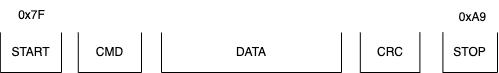
\includegraphics[width=14cm]{images/impedance_controler_software_measurement_protocol.png}
    \caption{Szabályozó szoftveres implementációjának egyszerűsített vázlata}\label{fig:measurement_protocol}
    \end{center}
\end{figure}
A START, CMD és STOP egy byte hosszúak. A DATA mező fix hosszúságú, legtöbb esetben 4 byte, de a CMD mezőtől függ.
A CMD mező kódolja a parancs típusát. A CRC mező a CMD és DATA mezők alapján számított 8 bites CRC, a kommunikációs 
hibákból eredő félrekonfiguráció esélyének csökkentéséért felel. 

A mérésekhez felhasznált egyéb eszközök a \ref{tab:measurement_tools}. táblázatban találhatóak.
\begin{table}[H]
    \small\centering
    \caption{További mérési eszközök}\label{tab:measurement_tools}
    \tabcolsep=1pt
    \begin{tabular}{l>{~}l>{~}l>{\quad}rl}
        \toprule
        \multicolumn{1}{c}{Eszköz neve} & \multicolumn{1}{c}{Gyártója} & \multicolumn{1}{c}{Típusa} & \multicolumn{2}{c}{Precizitás} \\ \midrule
        Mérőórás tolómérő & Berger & 020701-0007 & \(\pm\)0.02 & mm \\
        Digitális oszcilloszkóp & Rigol & DS1202Z-E & 200 MHz / 1 & GSa/s \\
        DC laboratóriumi tápegység & UNI-T & UTP3315TFL-II & 0-30V \(\pm\) 10 mV, 0-5A \(\pm\) 1 & mA \\
        Digitális multiméter & MAXWELL & MX-25304 & \(\pm\)0.1 mV - 1 V, \(\pm\) 0.1 \(\mu\)A - 10 & mA \\
        \bottomrule
    \end{tabular}
\end{table}

\section{Paraméter identifikáció}
A szabályozó megfelelő működésének feltétele, hogy rendelkezésre álljanak a motor pontos paraméterei. 
Bár az adatlapokból több szükséges paraméter is kiolvasható, vannak paraméterek, amiket külön kellett 
meghatározni. Ilyen a motorra terhelésként ráhelyezett propeller másodrendű nyomatéka és a viszkózus 
csillapítási tényező. A hajtómű áttétele, a rotor másodrendű nyomatéka és a nyomatékállandó esetében 
az adatlapokban szereplő értékek lettek alkalmazva. A rotor ellenállása és a motorvezérlő motorra adott 
feszültségjelének amplitúdója és a vezérlő parancs közötti viszony külön lettek meghatározva. 

A rotor ellenállásának meghatározásához egy sor állandó feszültség lett kapcsolva a motorra 
lefogott állapotban, és a motor által felvett áram került feljegyzésre. A mért értékek a \ref{tab:resistance_measurement}. 
táblázatban találhatóak. 
\begin{table}[H]
    \small\centering
    \caption{Ellenállás mérés adatok}\label{tab:resistance_measurement}
    \tabcolsep=5pt
    \begin{tabular}{d{-1}>{~}d{-1}}
        \toprule
        \multicolumn{1}{c}{Kapocsfeszültség [V]} & \multicolumn{1}{c}{Felvett áram [mA]} \\ 
        \multicolumn{1}{c}{(mind \(\pm\) 0.01)} &  \multicolumn{1}{c}{(mind \(\pm\) 0.1)}\\
        \midrule
        1.18 & 74.8 \\
        1.38 & 87.2 \\
        1.58 & 115.3 \\
        1.78 & 131.3 \\
        1.97 & 159.7 \\
        2.17 & 73.5 \\
        \bottomrule
    \end{tabular}
\end{table}

\section{Eredmények}

